%%%%%%%%%%%%%%%%%%%%%%%%%%%%%%%%%%%%%%%%%%%%%%%%%%%%%%%%%%%%%%%%%%%%%%%%%%%%%%%%%%%%%%%%%%%%%%%%%%%%%%%%
%%                                                                                                    %%
%% This is the source file for the official CAuDri-Challenge 202X regulations.                        %%
%%                                                                                                    %%
%% Can be compiled with PDFLaTeX, packages are strictly necessary.                                    %%
%% All graphics can be found on our OneDrive in CAuDri-Challenge\Regelwerk\202X\Source\graphics       %%
%%                                                                                                    %%
%%%%%%%%%%%%%%%%%%%%%%%%%%%%%%%%%%%%%%%%%%%%%%%%%%%%%%%%%%%%%%%%%%%%%%%%%%%%%%%%%%%%%%%%%%%%%%%%%%%%%%%%
\documentclass[a4paper]{report}

\title{CAuDri-Challenge Regulations \the\year{}}
\author{Max Weißer, Yannik Süssmuth}
\date{\today}

\usepackage{geometry}   	% Used to redfine page dimensions
\usepackage{lmodern} 	% Replaces 'computer modern' font style, better look on modern displays
\usepackage{fancyhdr} 	% Used for header and footer generation
\usepackage[]{graphicx}	% Include graphics
\usepackage{titlesec}	% Change properties of chapter/section titles
\usepackage{etoolbox}	% Used to extend functionality/properties of commands
\usepackage{color}		% Used for coloring letters and backgrounds
\usepackage{booktabs}	% Used for booktabs style (scientific looking) tables
\usepackage{parskip}		% Add spacing between paragraphs
\usepackage{float}		% Honestly, that's like the most important package
\usepackage{hyperref}	% Enables clickable links and references

% Page geometry
\geometry{hmargin=2.5cm,
          vmargin=1cm,
          headheight=1.5cm, 
          includeheadfoot}

% Define hyperref link colors
\hypersetup{colorlinks  = true,
            linkcolor   = black,
            urlcolor    = blue,
            citecolor   = black,
            anchorcolor = black}
            
% Helper dimension for colored boxes
\newlength\colorboxwidth
\setlength{\colorboxwidth}{\dimexpr\textwidth-2\fboxsep}

% Disable chapter text and change formatting of chapter titles (titlesec package)
\titleformat{\chapter}{\normalfont\huge\bf}{\thechapter.}{8pt}{\huge\bf}
\titlespacing{\chapter}{0pt}{-1\baselineskip}{1.5\baselineskip}

% Slightly scale the height of table rows 
\renewcommand{\arraystretch}{1.2}

% No indentation of new paragraphs
\setlength{\parindent}{0pt}

% Use Sans-Serif font as default
\renewcommand{\familydefault}{\sfdefault} 

% Use fancy headers (fancyhdr package)
\pagestyle{fancy}
% Enable headers on pages containing a new chapter (etoolbox package)
\patchcmd{\chapter}{\thispagestyle{plain}}{\thispagestyle{fancy}}{}{}
% Distance between header content and horizontal line
\renewcommand{\headruleskip}{2mm}
% clear existing header/footer entries
\fancyhf{}

% Header and footer definitions
\fancyhead[L]{\large CAuDri-Challenge Regulations \the\year{}}
\fancyhead[R]{
\includegraphics[width=3cm]{graphics/caudri_logo_no_border.jpg}\hspace{-5mm}
              \vspace{-3mm}}
\fancyfoot[L]{Page \thepage}
%\fancyfoot[R]{\leftmark} % Chapter name

\begin{document}

% Custom title page
\begin{titlepage}
	\makeatletter
	\begin{center}
	\vspace*{3cm}
	
	
\includegraphics[width=\textwidth]{graphics/caudri_logo_no_border.jpg}\\
	\vspace{1cm}
	
	\Huge\bfseries\@title\\
	\vspace{\baselineskip}
	
	\Large\@date\\
	\vspace{8cm}

	\large DISCLAIMER:\\
	
	{\raggedright This document may be subject to change up until the day of the competition.\\
	All changes will be announced on our Discord Server, in case of major changes we will inform all participants via E-Mail.\\
	New or removed features will be highlighted in \colorbox{yellow}{yellow}, differences to previous versions in \colorbox{green}{green}.\\}

	\end{center}	
	\makeatother
\end{titlepage}


\tableofcontents


\chapter{Overview} 

\section{Objectives}

The student competition “Cognitive Autonomous Driving (CAuDri) Challenge” provides a platform for student teams to get involved with the conceptualization and implementation of automated model vehicles. The challenge is to realize the best performing vehicle guidance system for different scenarios, which have been derived from requirements arising from a realistic environment. 

In the annual competition, participating students have the opportunity to present their know-how while competing with teams from other universities. 

\section{Tasks}

The student team is put in charge of developing, producing, and demonstrating a cost- and energy-efficient 1:10 concept for an automated vehicle by a fictional OEM. During the competition several driving tasks have to be executed as fast and precise as possible. In addition, the developed concept must be presented and explained. 

\section{Scoring}

Each concept and its realization will be assessed in comparison to the results of the other participating teams. For this, the teams compete in different dynamic events, while being awarded at most 700 points. 

The maximum amount of points is distributed to the different events as follows: 

\subsection{Dynamic Events}

\begin{table}[h]
\begin{tabular}{|l|l|}
\hline
Free Drive and Parking:  & 300 points \\ \hline
Obstacle Evasion Course: & 400 points \\ \hline\hline
Maximum Total Score:     & 700 points \\ \hline
\end{tabular}
\end{table}

\chapter{Competition}

\section{Organization}

The CAuDri-Challenge is organized and presented by the student teams “Smart Rollerz” (DHBW Stuttgart), “Team Spatzenhirn” (University of Ulm) and “KITcar e.V.” (Karlsruhe Institute of Technology). 

\section{Awards and Prizes}

The top student team of the CAuDri-Challenge will (presumably) be awarded with a plastic trophy. 

\section{Dates}

The CAuDri-Challenge annually takes place in October. (Due) dates will be published on the website. 

\section{Venue}

The CAuDri-Challenge will take place at the DHBW Stuttgart. (Lerchenstraße 1, 70174 Stuttgart) 

\section{Communication}

Teams can contact the CAuDri-Challenge organization team via the email address info@caudri-challenge.de. 

Furthermore, there exists an official Discord server for all participating teams:\\ \href{https://discord.gg/ZvPmWd5hAK}{https://discord.gg/ZvPmWd5hAK} 

\chapter{Regulations}

\section{Commission}

Rules and obligations of the CAuDri-Challenge can only be modified by the CAuDri-Challenge Regulations Commission. In cases of uncertainty or discrepancy the commission is responsible for official statements. 

\section{Validity of Regulations}

Only the regulations which have been published on the official website are valid for the competition. Old Regulations are invalidated, as soon as a new version of the regulations is published. Updates of the regulations will additionally be announced to registered teams. 

\section{Questions}

Every participant is obliged to thoroughly read, understand, and accept the regulations. In case of questions, the commission is to be consulted. Questions can either be directly posed to the commission or be published in the official CAuDri-Challenge Discord server regulations channel. 

Studying the regulations channel is recommended, as questions are being publicly discussed there on a regular basis. 

\section{Authority}

The commission can change the schedule or the regulations of the event at any time. All participants are obliged to cooperate with the commission and follow their instructions. 

\section{Limit of participating teams}

The commission reserves the right to limit the number of participating teams if this becomes necessary due to organizational reasons. In case of such a limit additional qualifying tasks may be requested from the teams. 


\chapter{Prerequisites for Attending}

Only students fulfilling the following conditions are allowed to participate in the CAuDri-Challenge. 

\section{Status of Enrollment}

Every participant must either be currently enrolled in a Bachelor’s, Master’s or a comparable degree program or the respective degree must not have been obtained more than six months before the competition. There is no restriction concerning the subject of study. Research staff and PhD students may not participate actively in conceptualization or development of the vehicle. They may not participate actively in the competition (cf. Section \ref{dev_know_how}).\\
{\colorbox{yellow}{No proof of enrollment will be necessary in 2024.}}


\section{Minimum Age}

\colorbox{yellow}{There is no minimum age for participation. Underage participants must submit a non formal written declaration of consent signed by their legal guardian.} 

\section{Number of Teams per Institution}

The number of teams per Institution is not limited. However, the development of the vehicles must be strictly separated. Software and hardware architectures of the respective teams must differ significantly. 

\section{Publication Rights}

By registering, every team and every participant declares their agreement with the publication of image, video and audio recordings. This also includes the recording of team presentations. This agreement might be revoked until the day of the competition. 

\chapter{Vehicle Requirements and Limitations}

The observance of the following regulations will be monitored during the competition. Violating these regulations will lead to a deduction of points or exclusion from the competition. The same vehicle must be used for all events. 

\section{Drivetrain}

The vehicle must be equipped with (an) electric motor(s). The number of driven wheels is not limited (torque vectoring is allowed). Other motors (e.g. combustion engines) are not permitted. 

\section{Energy Supply}

Energy must be supplied in the form of batteries. Changing the batteries between single events is allowed. 

\section{Physical Dimensions}

The vehicles must be based on four-wheeled 1:10 scale chassis. Only two axles are permitted. The wheelbase must measure at least 200 mm. The track width (measured from the center of the wheels) must measure at least 160 mm. The vehicle, including possible extensions and bodywork, must not be wider than 300 mm. The height of fixed installations must not exceed a height of 300 mm above the track surface. Flexible antennae are allowed.

Apart from this, the design of the chassis is subject to the team’s creativity, as long as it adheres the maximum physical dimensions. For the acceptance test, the car must be able to drive through a fixed gate (inner dimensions: height 300 mm, width 300 mm) in RC-mode. 

\section{Steering / Tires}

At least one axle must be steerable. Teams are expected to use cushion or foam rubber tires. Other types of tires need to be confirmed by the commission prior to the training sessions. The use of traction additives or studded tires is not allowed. 

\section{Sensor Setup}

The sensor setup can be arbitrarily chosen by the teams. Laser sensors are allowed only up to class 2 devices. 

\section{Data Transmission}

No data or signals must be transferred from the vehicle to the outside world during the dynamic events, except for those signals necessary for the remote control (cf. Section \ref{rc_mode}).\\
\colorbox{red}{\parbox{\colorboxwidth}{An active WiFi connection may be used during dynamic events, this will lead to a decreased score multiplier.(cf. Section \ref{freedrive_multipliers} and \ref{obstacle_multipliers})}}

\section{WiFi-Network}

\colorbox{green}{Each participating team may set up a single private wifi network.}\\
\colorbox{yellow}{\parbox{\colorboxwidth}{For internet access, participants can connect to the eduroam network at the venue.\\
(Removed: commission will set up a WiFi network)}}

\section{Bodywork}

The teams must be able to quickly disassemble the vehicles’ bodywork, so that the inner parts of the vehicle can be inspected at any time. The bodywork must conform to IP 10 (EN 60529). 

\section{RC-Mode} 
\label{rc_mode}

In emergency situations, the vehicle must be stoppable and maneuverable using a remote control. This can become necessary due to faults or errors in the data processing or due to other problems so that the vehicle cannot continue to execute its automated driving task. 

\subsection{Activating RC-Mode} 

RC-mode is activated by the remote control. An active RC-mode must be signaled by utilizing a sufficiently bright, flashing, blue light, which is visible from any position on the track. The light must be fixed at the highest point of the vehicle. The light must flash with a frequency of 1 Hz, showing a duty cycle of 50\%, beginning with the status "on" when activating RC-mode. RC-mode must only be activated after a clear misbehavior of the vehicle. This means e.g. completely leaving the designated course of the track. 

\subsection{Driving in RC-Mode}

Activation of RC-mode must instantly bring the vehicle to a complete halt, without further steering maneuvers. The vehicle must be in standstill for at least 1 s before it may be controlled with the remote control. During the events, the vehicle must not drive faster than 0.3 m/s forward and backward when RC-mode is engaged. However, the vehicle may be controlled directly after having stopped during training. Additional functionality is not allowed in RC-mode.
\bigskip\\
\colorbox{yellow}{Removed velocity limit of 1 m/s during Training}

\subsection{Transmission Frequencies} 

In order to limit interference between the vehicles of the different teams, each team must inform the commission about the transmission frequency of their remote control used when registering. Frequencies are issued on a first-come-first-serve basis. Additionally, specific models are known to interfere with Wi-Fi networks, or other infrastructure. Thus, remote controls using frequencies in the 2.4 GHz band need to be confirmed by the commission individually. 

\section{Handling of the Vehicle}

The vehicle must provide two distinctive buttons (e.g. push-buttons, touchscreen buttons, etc.), which start the different modes for the dynamic events. The buttons must be uniquely identifiable and easily reachable in order to allow non-team members (e.g. Judges, Referees) to start the vehicle. 

\section{Lights}

As in real traffic, lights shall signal different driving maneuvers. 

\subsection{Braking Lights} 

Three clearly visible and differentiable braking lights must be installed at the rear of the vehicle. Active braking must be signaled. 

\subsection{Direction Indicators}

Each corner of the vehicle must be equipped with a yellow / orange light. The respective lights at the correct side must be flashed at a maximum frequency of 2 Hz (50\% duty-cycle, initial state "on") when overtaking, turning, or parking. 

\subsection{RC-Mode-Indicator}

A clearly visible blue light is to be installed at the highest point of the vehicle, which flashes to signal the activation of RC-mode (cf. Section \ref{rc_mode}). 

\section{Development Know-How} 
\label{dev_know_how}

The basic concepts of the vehicle must be conceptualized and implemented by the students themselves. They must not accept the direct help of professional engineers or suppliers. The students are encouraged to do research and/or discuss their problems with professional engineers or suppliers. 

Ready-made solutions may never be included in the vehicle. This particularly concerns the use of predesigned algorithms which may be part of a hardware platform and serve the purpose of providing a fully functional system for perception, behavior generation or control for automated vehicles or robots. 

The final decision on acceptable components is taken by the commission. The teams are encouraged to contact the commission early in case of doubts or questions about a particular component. In case of violating these guidelines or intentional fraud, the commission has the right to exclude the respective team from the competition. 

\section{Safety Regulations}

During the competition, safety instructions issued by the venue and commission members are to be followed. Ignorance of notes or guidelines can be punished by excluding the respective team from the training sessions or the competition. Each individual is required at all times to take care that no other participants are injured or other vehicles are damaged due to careless behavior. 

As far as the sensor setup is concerned, special requirements and restrictions arise. All components within the vehicles must adhere to established guidelines for safe public usage. Particularly the usage of active sensors can be limited by this rule. 

The teams must make sure that no third parties are subject to possible injury due to installation or handling of the sensors. In case of questions concerning particular sensors, the admission must be discussed with the commission prior to the beginning of the training sessions. 

Violations of these regulations lead to an immediate exclusion from the competition. Any claim for compensation from the commission is excluded. 

\section{Modification of the Vehicle}

During the dynamic events, the hardware of the vehicle must not be modified except in case of supervised repair. The software must not be modified during the dynamic events. Changing and charging batteries is allowed. 

\chapter{Dynamic Events}

During the dynamic events, the actual performance of the automated model vehicles will be challenged in two different disciplines (Free Drive and Parking, Obstacle Evasion Course). Parking maneuvers are performed in a distinctive parking zone following the starting line during the “Free Drive” discipline. The additional elements of the “Obstacle Evasion Course” combine the rural road scenario with challenges of suburban scenarios. 

\section{Referees}

Referees around the track are evaluating each vehicle’s performance and will be responsible for registering violations. Team referees are nominated by every team to support the scoring during the dynamic events. Teams consisting of less than five members present during the dynamic events can choose to refrain from providing a referee. During dynamic events, team referees are the spokesperson for the commission and the official referees. Team referees are expected to approve the compliance of the track prior to the start of the individual discipline. Then, they will be asked to join a referee in observing a specific section of the track. The team referee has to stand back, while their own vehicle is on the track. 

\section{Free Drive (w/o Obstacles) and Parking}

In this event, the vehicle shall automatically cover the farthest possible distance in a given time. The vehicle drives in the right lane. Additionally, the vehicle can perform automatic parking maneuver by finding a suitable parking spot inside a parking lot. 

\subsection{Scenario}

The complexity of this scenario is limited. It consists of a road with two parallel lanes - one for each driving direction. This scenario shall imitate a rural road environment, consisting of long straight sections, tight turns, intersections, side road junctions and also containing a parking lot. The lanes are limited by different types of lane markings. All markings are white and approx. 18 mm to 20 mm wide, if not specified differently. The starting line (a checkered line of approx. 50 mm) marks the beginning of the track, which is the parking zone (cf. Section \ref{fig_parking_lot}). 

\subsubsection{Parking Lot}

Following the starting line and indicated by a traffic sign, there are parking areas containing spots for parking in parallel and perpendicular orientation to the track within the next 20 m. The parking zone is a planar and straight part of the track with a dashed center line without missing lane markings. Additional elements (intersections, missing lane markings, traffic signs, etc.) are not present. All areas for parking are located in this zone. 

\subsubsection{Parallel Parking}

Within the parking zone there is at least one parallel parking area next to the right lane. White cardboard boxes represent other vehicles. The boxes can be fixed to the ground. There is a space of 20 mm to 200 mm between the right lane marking and the side of the obstacle which faces the track. The obstacles measure at least 100 mm in height and length. The parking area and the track are located in the same ground plane. Individual parking spots of the parking area can be marked as no parking zones. These areas may not be used for parking, but may be used for maneuvering. 

There will be multiple parking spots of different size in the parallel parking area(s) next to the track. The left- and right-hand limits of the parking spots are defined by the right lane marking and an additional solid white line (also 18 mm to 20 mm wide). Front and rear limits are defined either by white cardboard boxes or by a no parking zone (cf. Section \ref{fig_parallel_parking}). Approaching from the starting line, the parking spots will be growing in length. The final and largest spot will beat least 700 mm in length. Nevertheless, small distances of under 400 mm might be present between obstacles anywhere inside the parallel parking area(s). 

\subsubsection{Perpendicular Parking}

An additional type of parking area within the parking zone consists of several parking spots with a perpendicular orientation to the track. Such area is located at least once on the left-hand side of the track and may also be used for parking. 

All spots have the same size, as shown in Section \ref{fig_perpendicular_parking}. The parking spots are separated and limited to the front as well as to the rear by 18 mm to 20 mm wide white markings. Parking spots can be blocked by obstacles or no parking zones. A parking spot is considered to be blocked, if the vehicle cannot be placed completely inside the spot. Obstacles possess the same dimensions as in the parallel parking area and can be placed at a distance of 20 mm to 100 mm from the solid left lane marking. 

For parking, the vehicle must be positioned inside one marked spot that is not blocked. Vehicles may move forward or backward into the parking space. The left lane of the track may only be crossed during the actual parking maneuver. When searching for a parking spot, the vehicle must continue to use the right lane. 

\subsubsection{Lane width}

Each lane has a width of 350 mm to 450 mm, measured from the inside of the respective markings. The left and right markings do not show lateral misalignments. However, the centerline may under circumstances (e.g. because of change of marking type, cf. next section) display lateral misalignments. 

\subsubsection{Lane markings}
\label{lane_markings}

Both lanes are separated by a dashed center line. The center line is interrupted every 200 mm for another 200 mm. This shape continues until reaching an intersection or the starting line, so that the center line might stop with a gap at these points. 

Alternatively to the dashed center line, a double solid line can be present. In this case the solid lines are spaced approx. 20 mm apart, yielding a total marking width of approx. 56 mm to 60 mm. A combination of a solid and a dashed line is also possible. In both cases, the inner edges of the markings define the width of the lane. Marking types can occur in arbitrary order. Marking types will persist for a distance of at least 1000 mm. There will be immediate changes between marking types (cf. Section \ref{fig_road_layout}). For the Free Drive event, these marking types are to be treated as regular dashed markings. 

The left and right track boundaries are given by solid white lines. On straight sections of the track, the outer track boundaries can also mark side road junctions. In this case, the outer track boundaries are marked with 100 mm long dashes, interrupted by 50 mm long gaps. These markings are to be treated as solid lines and must not be crossed, as the vehicle is assumed to have the right of way. 

Side road junctions may be at most 960 mm long. The junction is only marked by the change in marking types, there are no further markings for the side lane. Neighboring sections of the track are space at least 50 mm apart, measured from the outer edges of the markings. The minimal distance of the track to the end of the course area is 300 mm. The sharpest turn has an inner radius of 1000 mm. 

The circuit is mostly planar. Parts of the track can show slopes of up to 10\% (0.1 m difference in height on a length of 1 m). Uphill and downhill grades will be announced by traffic signs (cf. Section \ref{traffic_signs}). The signs will be placed at least 1000 mm prior to any change of slope. All of the lane markings can be missing at arbitrary locations for a maximum of 2000 mm \colorbox{red}{(2023: maximum of 800 mm).} Except for intersections, no more than two markings are missing at the same time. 

An example scenario is depicted in Section \ref{fig_example_circuit} in the appendix. 

In this event, no obstacles are located on the track. Possible stop lines and regulations concerning the right of way are to be ignored. 

\subsubsection{Traffic Signs}
\label{traffic_signs}

In addition to the parking sign at the starting line and the steep hill signs described above, other supporting traffic signs can be present on the roadside. 

Guide signs will be used to indicate sharp turns. They mark a curved section of the track with radii below 1200 mm, if it is located after a straight section of at least 3 m length. A first guide sign will be placed approx. 1.5 m before the transition to the turn. The second sign marks the beginning of the turn. Smaller signs will be repeated approximately every 400 mm until reaching the apex of the turn. 

Additional traffic signs can be present at the roadside. They are located on the right-hand side of the lane. For an exact specification see Section \ref{fig_traffic_signs}. In this event, regulations announced by traffic signs can be ignored. 

\subsubsection{Artifacts}
\label{artifacts}

The design of the area outside of the road is not defined. Artifacts in the form of objects or remainders of lane markings might be located outside of the road area. The minimum distance between artifacts and valid lane markings is 100 mm. 

\subsection{Execution of the Event}

\subsubsection{Start} 

The starting order of the teams will be announced by the commission, visualized using the start scheduling system (cf. Section \ref{start_scheduling}) during the competition. The vehicle must be placed in the start box, located next to the track (cf. Section \ref{start_box}). The attempt is started by a judge or a referee, signaled by the opening of the gate of the start box.

{\colorbox{yellow}{\parbox{\colorboxwidth}{It is not strictly necessary to detect the presence of the markings on the gate, the vehicle only has to detect when the gate is opened.(cf. Section \ref{fig_start_box_markings})}}

\subsubsection{Attempts} 

The attempt may be canceled while the gate of the start box is open. The team is then allowed a second attempt, after all other teams have completed their first attempt. Canceling an attempt is penalized (cf. Section \ref{freedrive_scoring}). A missed start results in a second attempt automatically. 

\subsection{RC-Mode}

In case the vehicle is not able to continue following the track on its own, the team may activate RC-mode in order to get the vehicle back into normal behavior. If the vehicle does not return into the right driving lane on its own, RC-mode must be activated immediately. Distances travelled outside of the driving lane will otherwise be subtracted from the total distance covered. Each activation of RC-mode is penalized. RC-mode is subject to the regulations in Section \ref{rc_mode}. 

\subsection{Parking}

Parking can be performed in any of the rounds of the Free Drive event. Successful parking maneuvers result in multipliers to the overall distance covered. Collisions during parking attempts result in penalties. The best parking results will be considered in the final score (i.e. additional parking maneuvers can eliminate penalties of other parking attempts). 

After each passing of the starting line, the vehicle can perform one parking attempt by finding a parking spot within the parking areas and maneuver into it, without touching the surrounding obstacles. The start of the parking maneuver has to be signaled using the turn indicators. After the vehicle came to a complete stop and flashed all turn indicators at least one time, signaling the end of the parking maneuver, it may drive on. The correct position of the vehicle will be checked from both sides of the track with the first flashing of the indicators. 

A complete parking maneuver requires the vehicle to come to a full stop being located in a valid spot with at least \colorbox{yellow}{three} of its wheels and flash all turn indicators at least one time. While maneuvering out of the parking spot, the vehicle may cross the left lane, but has to continue driving in the right lane. 

Leaving the outer boundaries of the parking area is penalized the same as leaving the right lane while driving. The speed in the parking lot is not limited, especially not after the parking maneuver has been completed. 

\subsection{Scoring}
\label{freedrive_scoring}

The covered distance under consideration of penalties will be multiplied by the achieved multiplier. The longest resulting distance will be awarded the maximum number of points. The subsequent teams will be scored in relation to the best team. 

\subsubsection{Timing}

Each team has 2 min to complete this event. Timing for the event starts with opening of the gate of the start box described in Section \ref{start_box}. 

\subsubsection{Penalties}
\label{freedrive_penalties}

\begin{table}[H]
\begin{tabular}{@{}lcc@{}}
\toprule
\textbf{Violation}                     			& \textbf{Maximum Count} & \textbf{Penalty} \\ \midrule
Leaving the right lane                 			& $\infty$               & 5m               \\
Activation of RC-mode                  			& $\infty$               & 5m               \\
Faulty activation of the brake light       	    & 3                      & \colorbox{yellow}{2.5m}       \\
False usage of turn indicators         			& 2                      & \colorbox{yellow}{2.5m}               \\
Vehicle not placed inside the markings 			& 2                      & 5m               \\
Collision with obstacle                			& 6                      & 5m               \\ 
\colorbox{yellow}{Driving in the wrong direction at an intersection}	& $\infty$               & 5m               \\\bottomrule
\end{tabular}
\end{table}

\subsubsection{Multipliers}
\label{freedrive_multipliers}

Each team starts this event with a multiplier of \textbf{1.0}. 

\begin{table}[H]
\begin{tabular}{@{}lcc@{}}
\toprule
\textbf{Triggering Event}         & \textbf{Maximum Count} & \textbf{Multiplier Modification} \\ \midrule
Canceled attempt / second attempt & 1                      & \colorbox{yellow}{-0.3}                             \\
\colorbox{yellow}{WiFi enabled during competition}   & 1   & -0.5 \\
Complete parking maneuver         & 2                      & +1.0                     
\\
\bottomrule
\end{tabular}
\end{table}

\section{Obstacle Evasion Course}

The event “Obstacle Evasion Course” extends the track of the Free Drive event with additional elements which need to be considered during the driving task. Parking maneuvers shall not be performed within this event. Static and dynamic obstacles are added to the rural road scenario. The track does additionally contain at least one suburban section at this point. All definitions concerning the course of the road maintain validity. There will be at least 1000 mm track length between obstacles. The additional elements are spaced at least 1000 mm apart aswell and do not overlap. Oncoming traffic is not to be expected, except when passing barred areas inside the suburban scenario. 

\subsection{Static Obstacles}

During this event, a number of static obstacles will be placed in the right lane, in the left lane and outside of the track. The body of each obstacle consists of white cardboard with dimensions as specified in the appendix (Section \ref{fig_obstacle_dimensions}). Obstacles can be fixed on the ground. The obstacles are not always placed exactly in a specific lane, however under no circumstance can both lanes be blocked. In this sense, static obstacles outside the track are no artifacts in the sense of Section \ref{artifacts}. Thus, the described minimum distance to lane markings for artifacts does not apply. 

Obstacles may force the vehicle to change lanes. Lane changes must be indicated using the turn indicators. Passing maneuvers must be executed without touching an obstacle. They must be completed after a maximum distance of 2 m after having passed the obstacle. 

\subsection{Dynamic Obstacles}

Apart from static obstacles, at least one dynamic obstacle is present on the track. Its shape resembles the static obstacles (“driving white cardboard box”) and it can be encountered in both lanes and in combination with other track elements, as long as this is not explicitly excluded. It moves at a speed of 0.6 m/s. Dynamic obstacles do not execute lane changes and do not perform any passing maneuver. Dynamic obstacles can stop temporarily and potentially block the right lane. It may be passed, but not in intersections. Passing maneuvers in intersections are penalized. A dynamic obstacle will not block both lanes in combination with a static obstacle, unless passing is prohibited in the area (cf. Section \ref{no_passing_zones}). Thus, allowed passing maneuvers can always be executed without encountering an obstacle on the left lane. The passing maneuver is subject to the same regulations as when passing a static obstacle. 

\subsection{Intersections of the Rural Road Scenario}
\label{intersection_rural}

Sections of the track can be part of intersections with other parts of the track. The respective lanes meet at angles between 70° and 90°. 

An intersection possesses three to four entries or exits respectively. Design and layout of the intersections of the rural road scenario are shown in the appendix (Section \ref{intersection_rural}). Left and right lane boundaries of intersecting lanes can be connected through a rounded transition with a radius of about 100 mm. Intersections of the rural road scenario must be crossed driving straight. Entries to intersections can display stop lines. These lines are 36 mm to 40 mm wide and cross one lane completely.

Additionally, a stop line is complemented by a traffic sign (stop sign, cf. Section \ref{fig_traffic_signs}). Entries without a stop line are not marked separately. The right of way is only announced by the respective traffic sign. If a stop line is located in the own lane, the vehicle must stop for at least 3 s. The front of the vehicle must be located in front of the stop line, however the distance must not be greater than 150 mm. 

The right of way of a dynamic obstacle must be respected at an intersection, if the dynamic obstacle is located within the defined area (cf. Section \ref{fig_intersection_give_way}). If the vehicle does not possess the right of way, it must wait until the dynamic obstacle has completely crossed the intersection. Only one dynamic obstacle at a time can be present at an intersection. 


\subsection{No-Passing Zones}
\label{no_passing_zones}

Sections of the track, not only in the suburban area, can be defined as no-passing zones. Corresponding traffic signs and lane markings will indicate such sections (cf. Section \ref{lane_markings}). In sections with a solid center line (a solid line within a double center line facing the ego lane) obstacles must not be passed. However, if a passing maneuver has been started before a no-passing zone, the vehicle is allowed to return to the right lane in any case. 

In a no-passing zone, the dynamic obstacle must be followed at a distance of at least 300 mm until the end of the zone. Static obstacles will not block the right lane in no-passing zones. Since passing is prohibited, a combination of adynamic obstacle in the right lane and a static object in the left lane can occur, temporarily blocking the whole track. 

\subsection{Two-lane Expressway}

Sections of the rural scenario, can be defined as an expressway. The beginning and end of such sections will be indicated by traffic signs (cf. Section \ref{fig_traffic_signs}). Expressways are a planar and mostly straight section of at least 10 m length, without any sharp turns. Any distinctive curve will be supported with traffic signs, as described in Section \ref{traffic_signs}. Vehicles on the expressway have right of way, no stop lines will be encountered. No obstacles will be present in the right lane of this section. Since the track is assumed to be a two-lane expressway, the vehicles must stay in the right lane all the time.  

\subsection{Suburban Scenario}

\subsubsection{Beginning and End of the Suburban Scenario}

The suburban area is a special section of the track, containing additional elements compared to the track design of the rural road scenario. Beginning and end of suburban areas are defined by markings on the road surface (cf. Section \ref{fig_road_markings}) and according traffic signs (cf. Section \ref{traffic_signs}). 

The speed limit within the suburban section, as indicated by the traffic signs has to be scaled by 1:10 (i.e. a speed limit of 30 km/h corresponds to 0.83 m/s). In addition to the speed limits depicted in the signs marking the suburban scenario, other numeric signs in steps of 10 km/h might appear (e.g. a speed limit of 20 km/h). Speed limit zones begin and end at the road markings, as depicted in Section \ref{fig_speed_limit_zone}. The according traffic signs will be placed at those positions. Elements of the suburban scenario will not be located on uphill and downhill grades. 

\subsubsection{Traffic Signs}

In addition to the traffic signs defined in Section \ref{traffic_signs} and \ref{intersection_rural}, the suburban scenario contains several other traffic signs which must be respected. Each traffic sign defines the beginning of the connected elements as defined in the following sections. Traffic signs can only occur in combination with their connected element. The exact dimensions and positioning are defined in the appendix of this document (cf. Section \ref{fig_traffic_signs}). Distances for longitudinal distances are measured on the right hand lane marking. Each Traffic Sign of the suburban scenario is complemented with specific markings on the road surface. Those markings must not have the same distance to the corresponding element as the traffic sign (cf. Section \ref{turning}). See the following sections for the according specifications. 

\subsubsection{Barred Area}

In addition to obstacles, the suburban scenario can contain barred areas on straight sections of the track. These areas block one lane for a length of max. 2000 mm, measured along the outer lane marking. The areas must be passed just as a regular obstacle. Barred areas are marked with a18 mm to 20 mm wide trapezoidal outline, filled with 36 mm to40 mm wide white markings with black spacing. For shape and dimensions see Section \ref{fig_barred_area}. The areas are at least 150 mm wide and are always connected with the left or right lane boundaries. Oncoming traffic has the right of way at barred areas, indicated by a corresponding traffic sign (cf. Section \ref{fig_traffic_signs}). 

If a dynamic obstacle is located within 1000 mm of the beginning of the barred area, the vehicle has to wait. Switching lanes is only allowed with an empty left lane, oncoming traffic must have completely passed. The desired passing maneuver has to be indicated while waiting by flashing the left turn indicators. Only one dynamic obstacle at a time can occur at a barred area. If the vehicle is able to pass a barred area without leaving the own lane or driving over the markings, the vehicle may continue along the barred area even in case of oncoming traffic. 

\subsubsection{Crosswalk}

In a suburban area, one or more crosswalks may be present. These are marked with several 36 mm to 40 mm wide and 400 mm long white markings parallel to the direction of travel which are spaced 40 mm apart (cf. Section \ref{fig_crosswalk}). A crosswalk is indicated by a corresponding traffic sign (cf. Section \ref{fig_traffic_signs}). On the roadside at each crosswalk “pedestrians” may wait to cross the road. For this purpose two areas are defined which may contain relevant pedestrians. 

A “pedestrian” is depicted by a small white cardboard box in analogy to the static obstacles. In addition, each pedestrian is marked with a pictograph, in order to facilitate its detection (cf. Section \ref{fig_pedestrians}). Multiple pedestrians can be located on the right- as well as on the left-hand side of the crosswalk. Pedestrians will always be clearly distinguishable from the view of the approaching vehicle. Only if at least one pedestrian is present in the defined zones, the vehicle must stop in front of the crosswalk. Stopping must be performed with the same regulations as at intersections. Pedestrians start crossing the street only after the vehicle has stopped. If all relevant pedestrians have crossed in front of the vehicle, the vehicle may continue. Driving on before all pedestrians start to cross and have cleared the right lane will be penalized as collisions with obstacles. 
\bigskip\\
\colorbox{yellow}{Pedestrian island was removed} 

\subsubsection{Extended Regulations at Intersections}

In addition to the requirements arising from stop lines, there can be different regulations for the right of way at intersections in the suburban scenario. Three types of intersections have to be considered: 

\begin{itemize}
\item Intersections with stop lines (cf. Section \ref{intersection_rural}) 
\item Intersections with priority road and give-way lines 
\item Intersections without regulations by road markings or signs (priority to the right)
\end{itemize}

Dimensions and layout of the additional intersections are displayed in the appendix (cf. Section \ref{additional_intersections}). Stop lines and give-way lines at priority roads are also announced by traffic signs (cf. Sections \ref{fig_traffic_signs}). A give-way line is 36 mm to 40 mm wide and consists of 80 mm long dashes, interrupted by 60 mm long gaps. Stop and give-way lines occur in pairs at opposing intersection entries, unless the priority road displays a mandatory direction and requires turning (cf. next Section). At a give-way line, the vehicle must stop for at least 1 s. 

Dynamic obstacles must be considered in any type of intersection. If an intersection does not contain any indication of priority by road markings or signs, priority to the right is to be applied. There will be no traffic signs to announce such intersections, while all four arms of the intersection will display a give-way line. The requirement to stop and potentially give the right of way to dynamic obstacles must still be respected. Scenarios which yield ambiguous regulations of the right of way will not be encountered. 

\subsubsection{Turning}
\label{turning}

In addition to the intersections described above, intersections in the suburban scenario can have a mandatory direction to cross the intersection. Different scenarios are shown in Section \ref{fig_intersection_mandatory}. This will be announced by a corresponding traffic sign and a marking on the road surface (cf. Sections \ref{traffic_signs} and \ref{fig_road_markings}). Vehicles will have to turn left or right according to these regulations. In the intersection, the mandatory direction will additionally be indicated by dashed turn lines that continue the center line and the right lane boundary. Turn lines cannot be missing. 

\subsubsection{Speed Control}

Within a suburban area, the vehicle has to adhere to the given speed limit. Devices for controlling the speed of the vehicle might be present. 

\subsection{Execution of the Event}

\subsubsection{Start}

The starting order of the teams will be announced by the commission, visualized using the start scheduling system (cf. Section \ref{start_scheduling}) during the competition. The vehicle must be placed in the start box, located next to the track (cf. Section \ref{start_box}). The attempt is started by a judge or a referee, signaled with opening of the gate of the start box.\\
{\colorbox{yellow}{\parbox{\colorboxwidth}{It is not strictly necessary to detect the presence of the markings on the gate, the vehicle only has to detect when the gate is opened.(cf. Section \ref{fig_start_box_markings})}}


\subsubsection{Attempts}

The attempt may be canceled while the gate of the start box is open. The team is then allowed a second attempt, after all other teams have completed their first attempt. Canceling an attempt is penalized (cf. Section \ref{obstacle_scoring}). A missed start results in a second attempt automatically. 

\subsection{RC-Mode}

In case the vehicle is not able to continue following the track on its own, the team may activate RC-mode in order to get the vehicle back into normal behavior. If the vehicle does not return into the right driving lane on its own, RC-mode must be activated immediately. Distances travelled outside of the driving lane will otherwise be subtracted from the total distance covered. Bonuses cannot be earned by vehicle behavior shown in RC-mode. Additionally, skipping challenges of the obstacle course (by not driving in the right lane) will be punished with the penalty designated for the respective element. Each activation of RC-mode is penalized. RC-mode is subject to the regulations in Section \ref{rc_mode}. 

\subsection{Scoring}
\label{obstacle_scoring}

The covered distance under consideration of penalties will be multiplied by the achieved multiplier. The longest resulting distance will be awarded the maximum number of points. The subsequent teams will be scored in relation to the best team. 

\subsubsection{Timing} 

Each team has 2 min to complete this event. Timing for the event starts with opening of the gate of the start box described in Section \ref{start_box}. 

\subsubsection{Penalties} 

\begin{table}[H]
\begin{tabular}{@{}lcc@{}}
\toprule
\textbf{Violation}                                                 & \textbf{Maximum Count} & \textbf{Penalty}\\ \midrule
Leaving the right lane (more than one wheel)                       & $\infty$               & 5m               \\
Activation of RC-mode                                              & $\infty$               & 5m               \\
Stopping outside of the 150 mm area at intersections or crosswalks & $\infty$               & 5m               \\
Collision with an obstacle                                         & $\infty$               & 5m               \\
Violating safety distance to dynamic obstacle                      & $\infty$               & 5m               \\
Too long passing maneuver                                          & $\infty$               & 5m               \\
Starting a passing maneuver in intersection                        & $\infty$               & 5m               \\
Passing pedestrian islands in the wrong lane                       & $\infty$               & 5m               \\
Falsely using turn indicators                                      & 3                      & \colorbox{yellow}{2.5m}                \\
\colorbox{yellow}{Driving in wrong direction at intersection}      & $\infty$               & 5m               \\ \bottomrule
\end{tabular}
\end{table}

\subsubsection{Multipliers}
\label{obstacle_multipliers}

Each team starts this event with a multiplier of 1.0. 

\begin{table}[H]
\begin{tabular}{@{}lcc@{}}
\toprule
\textbf{Triggering Event}                        & \textbf{Maximum Count} & \textbf{Multiplier Modification} \\ \midrule
Canceled attempt / second attempt                & 1                      & \colorbox{yellow}{–0.3}         \\
\colorbox{yellow}{WiFi enabled during competition} & 1    & -0.5 \\
Right of way respected                           & $\infty$               & + 0.2                            \\
Waited for all crossing pedestrians at crosswalk & $\infty$               & + 0.2                            \\
Barred area respected                            & $\infty$               & + 0.2                            \\
Barred area respected                            & $\infty$               & + 0.2                            \\
No-passing zone respected                        & $\infty$               & + 0.2                            \\ 
\bottomrule
\end{tabular}
\end{table}

\chapter{Competition Schedule} 

In this chapter, the general schedule execution of the competition is described. 

\section{Training} 

In order to guarantee safe and fair training conditions, the training sessions are divided into time slots. The number of teams allowed on the track at the same time and the length of the slots will be announced on the website before the competition. The commission might change the slots and the number of teams on the track without further notice. In case of clear violations of training slots, the commission may issue penalties which will be subtracted from the final score of the respective teams. In case of repetitive violations of slots or if team members endanger other teams or their equipment, the commission may expel single team members or whole teams from the competition. 

\section{Qualifying}

\colorbox{yellow}{There will be no qualifying in \the\year{}.} 

\section{Competition} 

\colorbox{yellow}{The follwing chapter is only for future reference.}\\ 
\colorbox{yellow}{The \the\year{} CAuDri-Challenge schedule will differ from the one described below.}

\subsection{Preparations} 

30 min before the beginning of the competition, the teams must hand in their vehicles at the “parc fermé”. No modifications of the vehicles must be made after this point. Batteries must be separated from the system, the vehicle must be switched off. All external tools must be removed from the vehicle, all wireless communication on board the vehicles (Wi-Fi, Bluetooth, etc.) must be switched off or removed, except for the remote control communication. The remote control must be placed next to the vehicle in switched off state. When handing in the vehicle, the teams must make a definite statement to the head referee in which events they would like to participate. This is to ensure a smooth execution of the competition. 

\subsection{Start Scheduling System}
\label{start_scheduling}

A traffic-light-like start scheduling system will signal the teams when to pick up their vehicle at the “parc fermé” and begin to prepare for starting. The traffic light will show the following stages: 

\begin{itemize}
\item 1. Red: No preparation necessary 

\item 2. Yellow: The vehicle must be prepared for the start. The team picks up their vehicle at the “parc fermé”. Time budget for preparation is 5 min. The teams may change to fully charged batteries in this context. However, no additional preparation (using external tools) is allowed at this stage. The idle, but ready, vehicle must be brought to the start box at this point. Timing will start, regardless whether the vehicle is ready or not. 

\item 3. Green: When showing “green” the gate of the start box might open at any time. After each event, the vehicle must be returned to the “parc fermé” immediately. Batteries must again be separated from the system, the vehicle must be switched off. The remote control must be placed next to the vehicle in switched off state. 
\end{itemize}

\subsection{Start Box}
\label{start_box}

The start box is separated from the track by physical barriers. Up to two team members are allowed to prepare the start of the vehicle in the start box. To the front of the start box is an openable gate, marked with a traffic sign and a matrix barcode (cf. Section \ref{fig_start_box_markings}). An attempt starts with the opening of the gate. The start box exit can be separated from the track by a solid white line. This line may be crossed to enter the track. The gate of the start box remains open for 30 s. An attempt is canceled if: 

\begin{itemize}
	\item The vehicle has not been placed ready to start in the box when the gate opens,
	\item The gate is forced open by a vehicle

	\item The vehicle fails to leave the box while the gate is open 

	\item RC-mode is activated inside the start box
\end{itemize}

Penalties will not be applied until the vehicle passes the start line (i.e. collisions in the start box or driving outside of the right lane before passing the start line do not reduce the overall score). 

%\subsection{Order of Events}
%
%\colorbox{red}{TODO}
%
%As described, “Carolo-Master-Cup” and “Carolo-Basic-Cup” do not share the same track. Thus, the teams of the “Carolo-Basic-Cup” will perform their dynamic events on parallel tracks initially. In case of a large number of participating teams, the dynamic events of the “Carolo-Basic-Cup” may be performed individually, prior to the official evening event of the “Carolo-Cup”. Subsequently, the competition area will be converted to a large circuit for the dynamic events of the “Carolo-Master-Cup”. The first event of both competitions is the “Free Drive and Parking”: One team after another starts its event according to the regulations in Section 5.2. The order of teams within each competition is fixed. The calls for preparation and start are made according to the start scheduling system, described above. In both competitions, the event “Obstacle Evasion Course” will follow next. The starting order will stay the same as in “Free Drive and Parking”. The first attempt can be canceled according to the regulations in Sections 5.2.2.2 and 5.3.7.2. The respective team is moved to the end of the schedule and will be called again to attempt a second run. 

 
\appendix
\chapter{Appendix}
If not indicated differently, dimensions and angles specified in the figures have a tolerance of
±5\%. Unless otherwise noted, all dimensions are in millimeters (mm).
Dimensions and angles defined in the previous chapters may not be repeated in the figures.

\section{Parking Lot}
\label{fig_parking_lot}
\begin{figure}[H]
\begin{center}
	\centering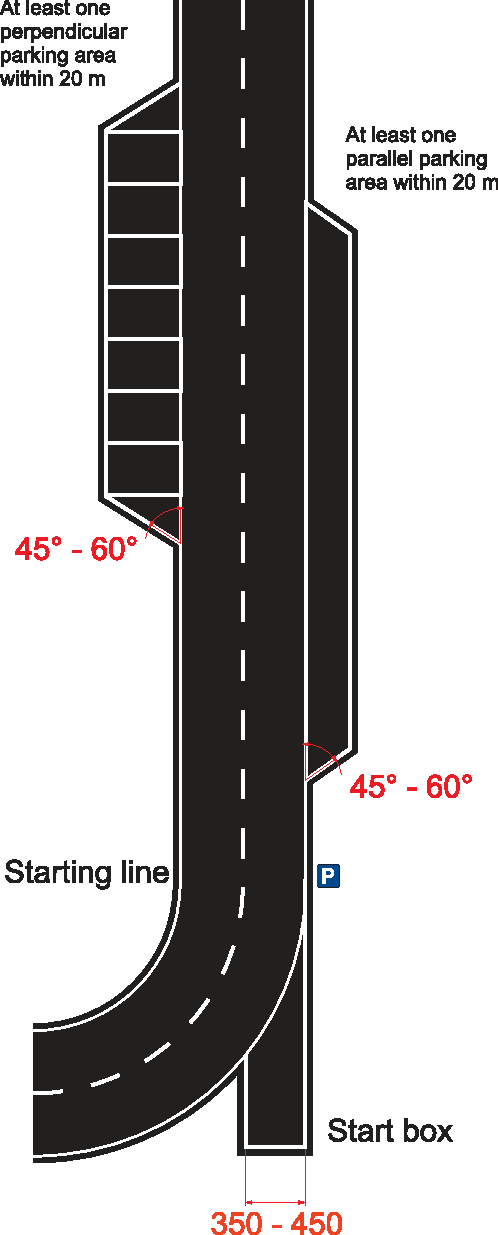
\includegraphics[scale=0.8]{graphics/Abb_1_parking_lot.pdf}
\end{center}
\end{figure}

\section{Parallel Parking}
\label{fig_parallel_parking}
\begin{figure}[H]
\begin{center}
	\centering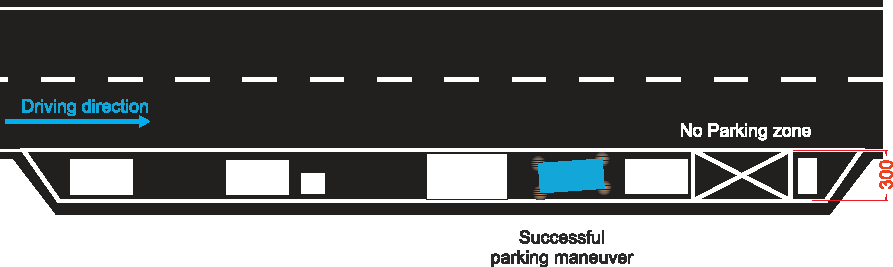
\includegraphics[]{graphics/Abb_2_parallel_parking.pdf}
\end{center}
\end{figure}

\section{Perpendicular Parking}
\begin{figure}[H]
\label{fig_perpendicular_parking}
\begin{center}
	\centering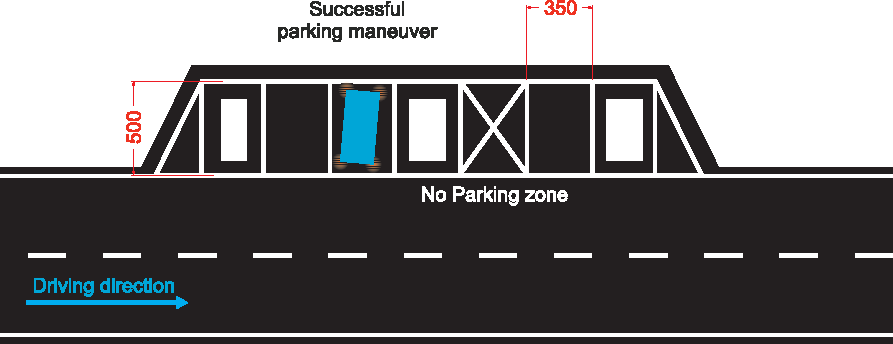
\includegraphics[]{graphics/Abb_3_perpendicular_parking.pdf}
\end{center}
\end{figure}

\section{Road Layout and Lane Markings}
\label{fig_road_layout}
\begin{figure}[H]
\begin{center}
	\centering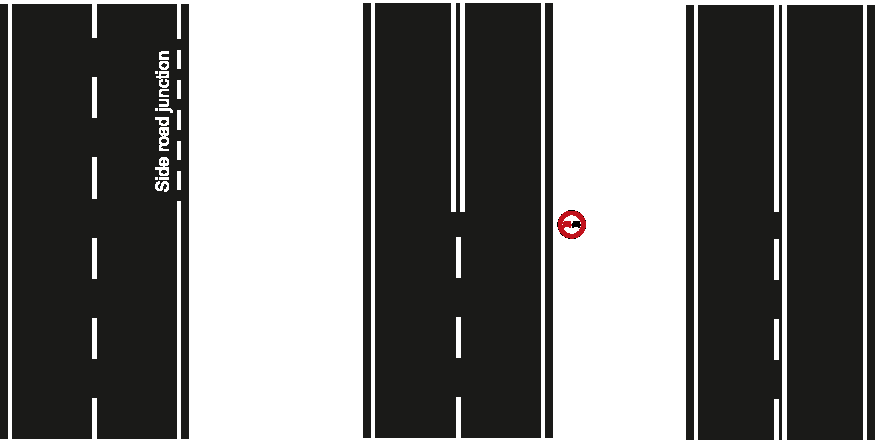
\includegraphics[]{graphics/Abb_4_road_layout.pdf}
\end{center}
\end{figure}

\section{Intersection of the Rural Road Scenario}
\label{fig_intersection_rural}
\begin{figure}[H]
\begin{center}
	\centering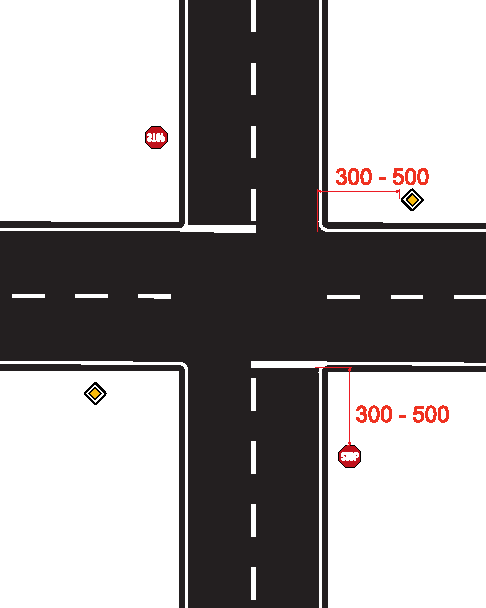
\includegraphics[]{graphics/Abb_5_intersection.pdf}
\end{center}
\end{figure}

\subsection{Dynamic Obstacles at Intersections - Give-Way Condition}
\label{fig_intersection_give_way}
\begin{figure}[H]
\begin{center}
	\centering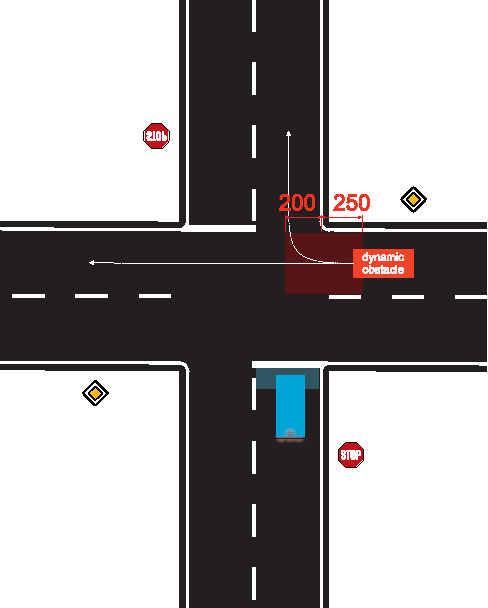
\includegraphics[]{graphics/Abb_6_intersection_give_way.pdf}
\end{center}
\end{figure}

\section{Speed Limit Zone}
\label{fig_speed_limit_zone}
\begin{figure}[H]
\begin{center}
	\centering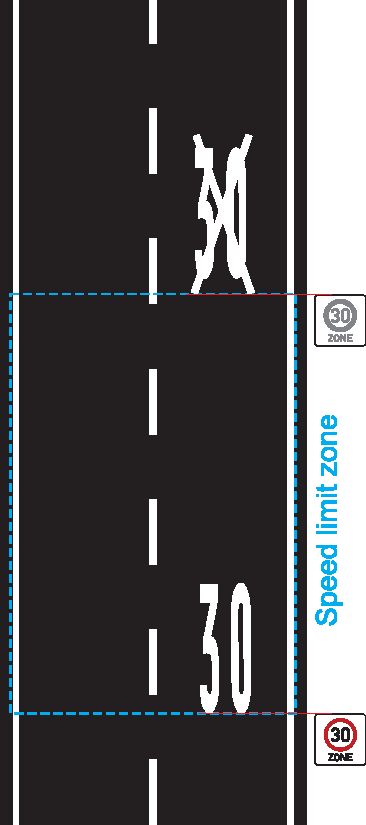
\includegraphics[]{graphics/Abb_7_speed_limit_zone.pdf}
\end{center}
\end{figure}

\section{Barred Area}
\label{fig_barred_area}
\begin{figure}[H]
\begin{center}
	\centering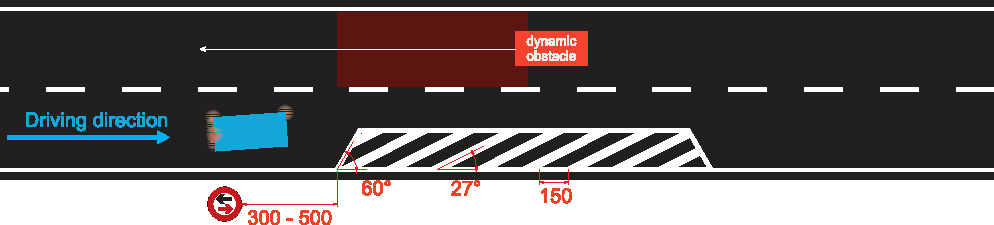
\includegraphics[width=\textwidth]{graphics/Abb_8_barred_area.pdf}
\end{center}
\end{figure}

\section{Crosswalk}
\label{fig_crosswalk}
\begin{figure}[H]
\begin{center}
	\centering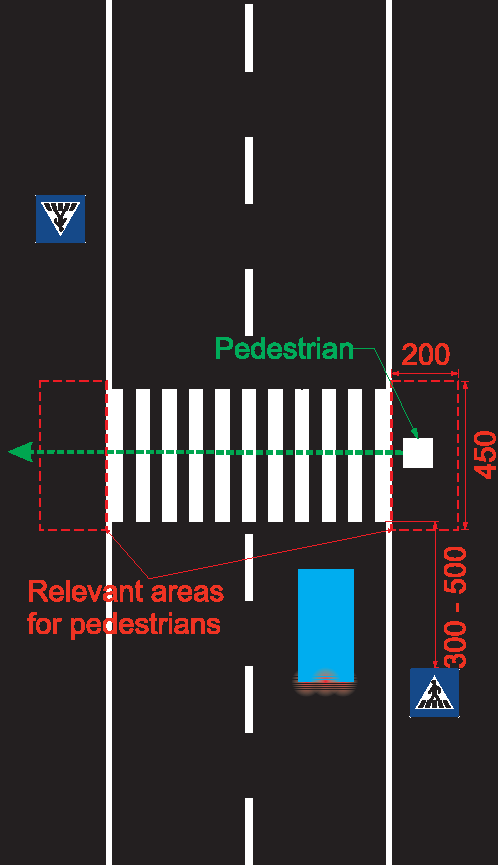
\includegraphics[]{graphics/Abb_9_crosswalk.pdf}
\end{center}
\end{figure}
\newpage

\section{Pedestrian Island}
\colorbox{yellow}{\large Deprecated}
\begin{figure}[H]
\begin{center}
	\centering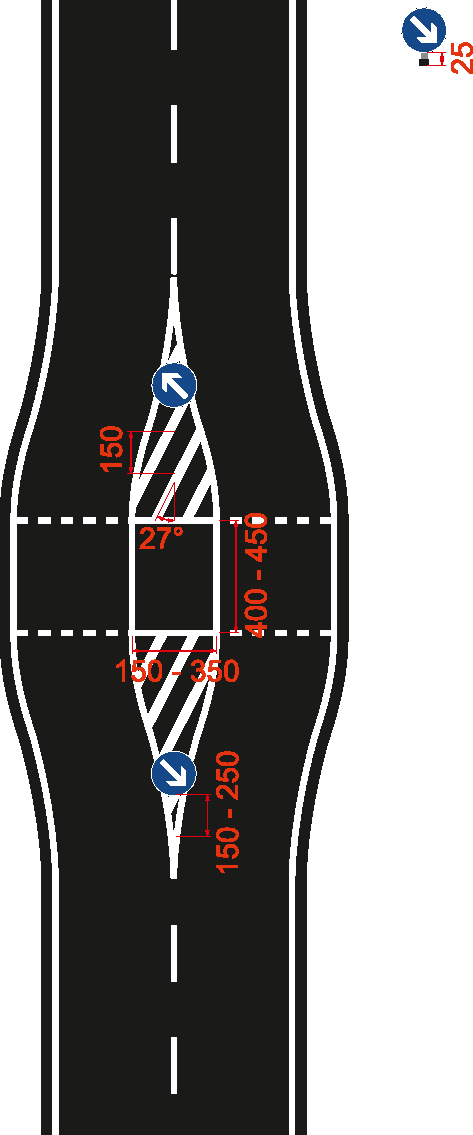
\includegraphics[]{graphics/Abb_10_pedestrian_island.pdf}
\end{center}
\end{figure}
\newpage

\subsection{Pedestrian Island with Crosswalk}
\colorbox{yellow}{\large Deprecated}
\begin{figure}[H]
\begin{center}
	\centering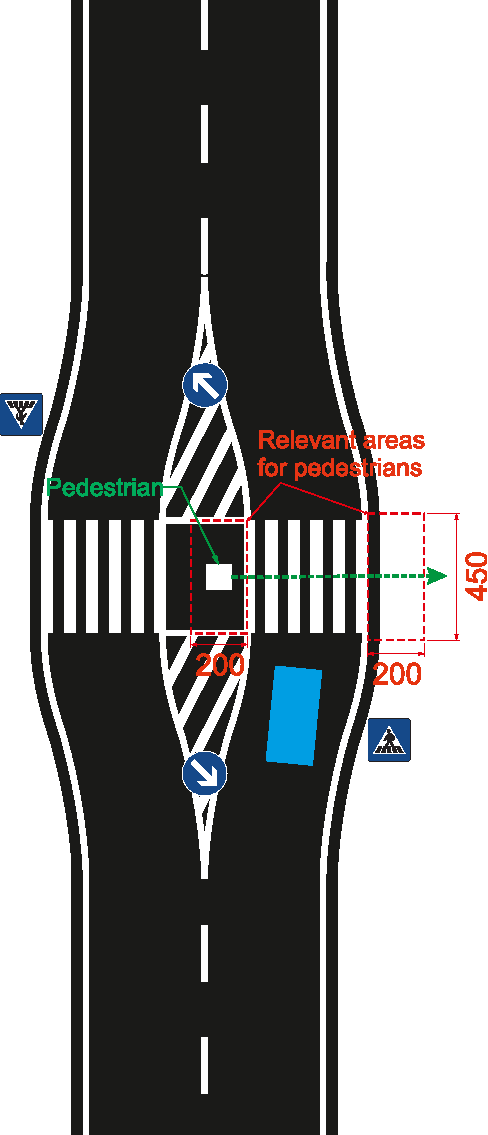
\includegraphics[]{graphics/Abb_11_pedestrian_island_crosswalk.pdf}
\end{center}
\end{figure}

\section{Additional Intersections of the Suburban Scenario}
\label{additional_intersections}

\subsection{Intersection with Give-Way Lines}
\label{fig_intersection_give_way_lines}
\begin{figure}[H]
\begin{center}
	\centering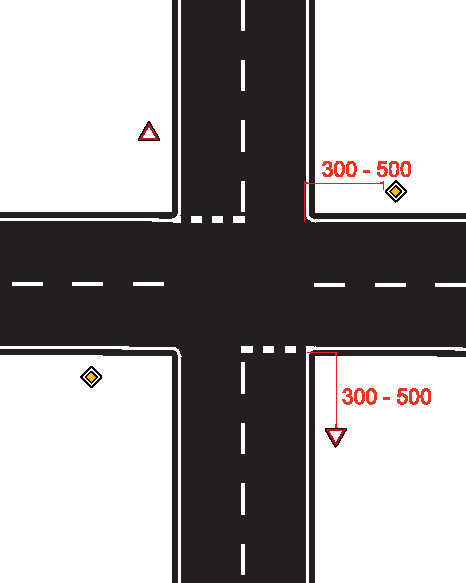
\includegraphics[]{graphics/Abb_12_intersection_give_way_lines.pdf}
\end{center}
\end{figure}

\subsection{Intersection with Priority to Right}
\label{fig_intersection_priority}
\begin{figure}[H]
\begin{center}
	\centering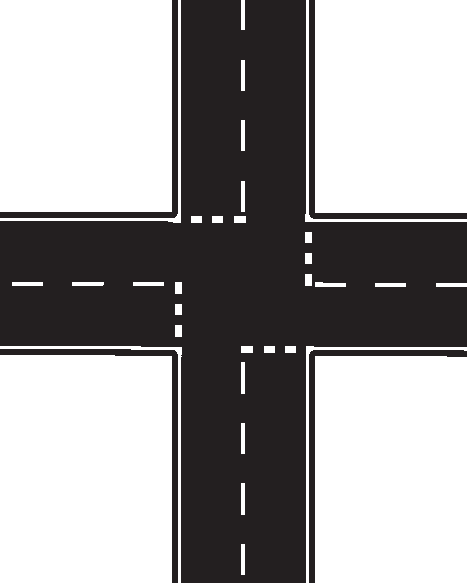
\includegraphics[]{graphics/Abb_13_intersection_priority.pdf}
\end{center}
\end{figure}

\subsection{Intersection with Mandatory Turn}
\label{fig_intersection_mandatory}
\subsubsection{Mandatory Crossing Direction - Stop Condition}
\begin{figure}[H]
\begin{center}
	\centering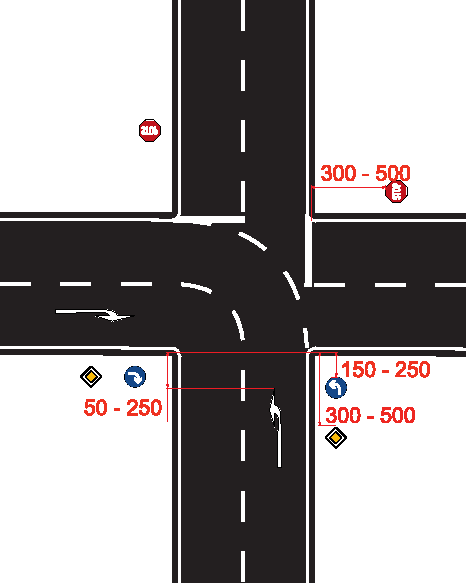
\includegraphics[]{graphics/Abb_14_mandatory_stop.pdf}
\end{center}
\end{figure}

\subsubsection{Mandatory Crossing Direction - Give-Way Condition}
\begin{figure}[H]
\begin{center}
	\centering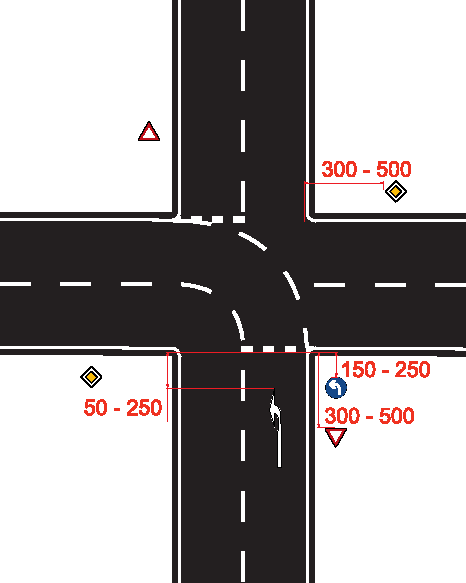
\includegraphics[]{graphics/Abb_15_mandatory_give_way.pdf}
\end{center}
\end{figure}

\subsubsection{Mandatory Crossing Direction - Right of Way Condition}
\begin{figure}[H]
\begin{center}
	\centering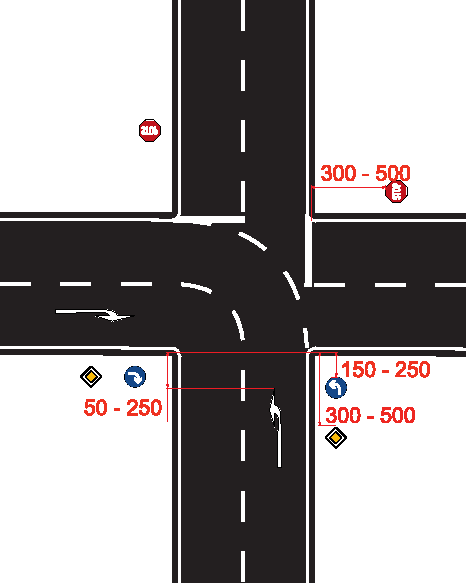
\includegraphics[]{graphics/Abb_16_mandatory_right_of_way.pdf}
\end{center}
\end{figure}

\section{Road Markings}
\label{fig_road_markings}
\begin{figure}[H]
\begin{center}
	\centering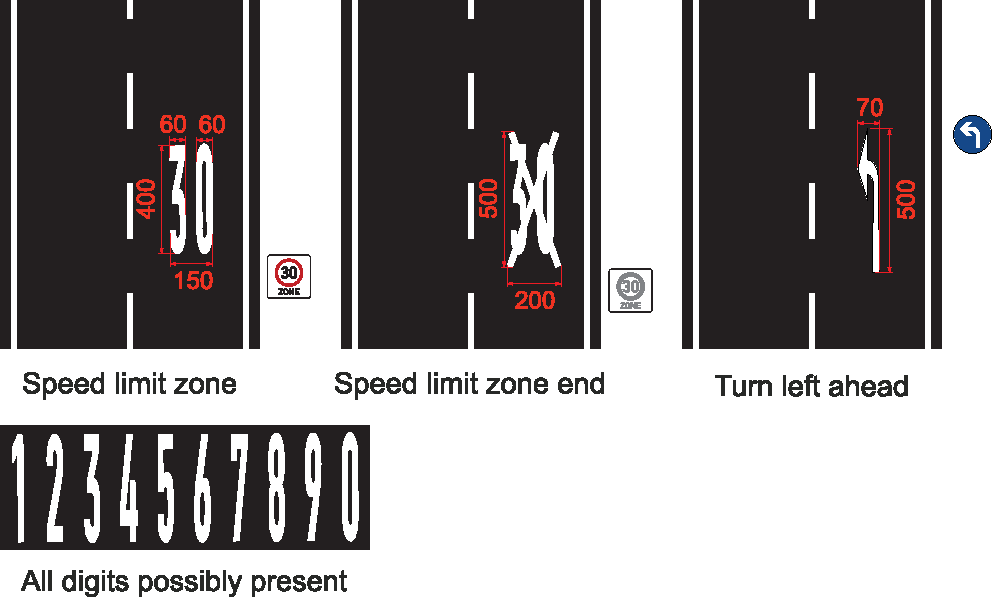
\includegraphics[width=\textwidth]{graphics/Abb_17_road_markings.pdf}
\end{center}
\end{figure}

\section{Traffic Signs}
\label{fig_traffic_signs}
\subsection{Definition of Traffic Signs}
The traffic signs are defined according to StVO (Legal definition of traffic rules) and are applied as described there, except otherwise defined in this document. Additional information about the dimensions can be scaled based on this source.

Traffic signs might appear in their mirrored version as well, e.g. turning symbols can indicate right or left turns.

\begin{figure}[H]
\begin{center}
	\centering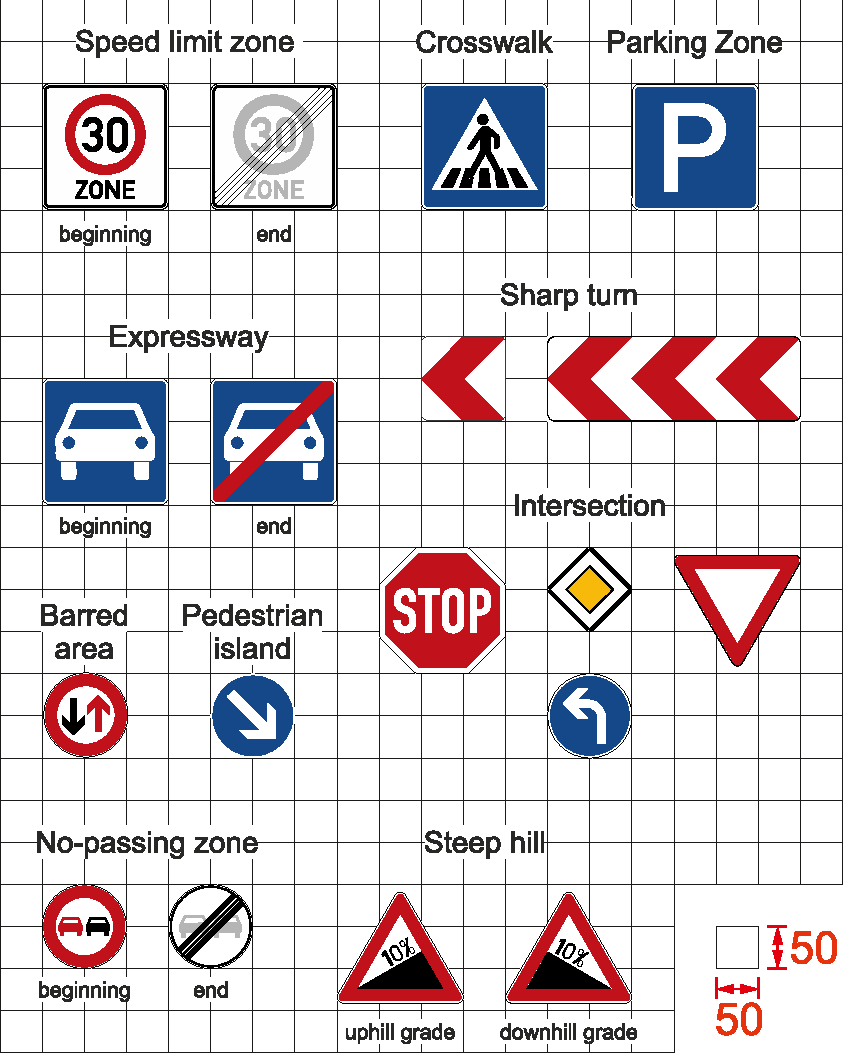
\includegraphics[]{graphics/Abb_18_traffic_signs.pdf}
\end{center}
\end{figure}

\subsection{Positioning of Traffic Signs}
\begin{figure}[H]
\begin{center}
	\centering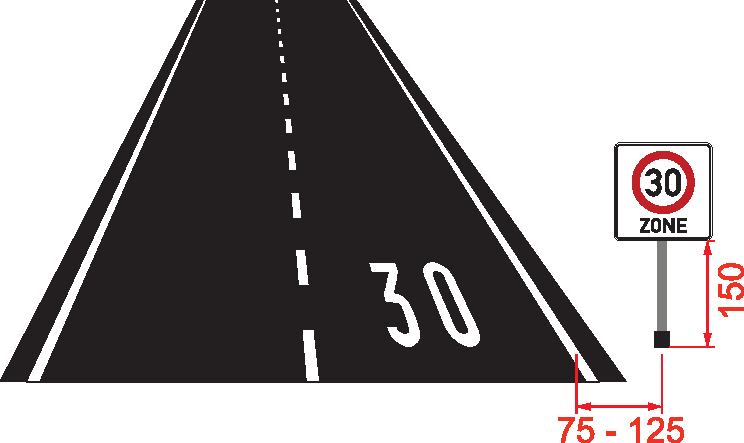
\includegraphics[]{graphics/Abb_19_positioning_of_traffic_signs.pdf}
\end{center}
\end{figure}

\section{Dimensions of Obstacles}
\subsection{Static and Dynamic Obstacles on the Track}
\label{fig_obstacle_dimensions}
\begin{figure}[H]
\begin{center}
	\centering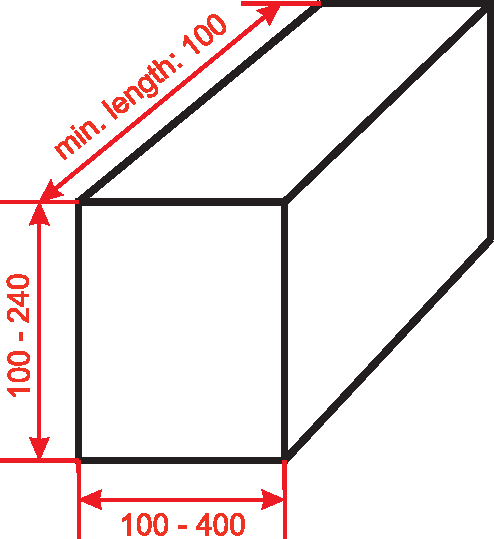
\includegraphics[]{graphics/Abb_20_obstacles.pdf}
\end{center}
\end{figure}

\subsection{Pedestrians}
\label{fig_pedestrians}
\begin{figure}[H]
\begin{center}
	\centering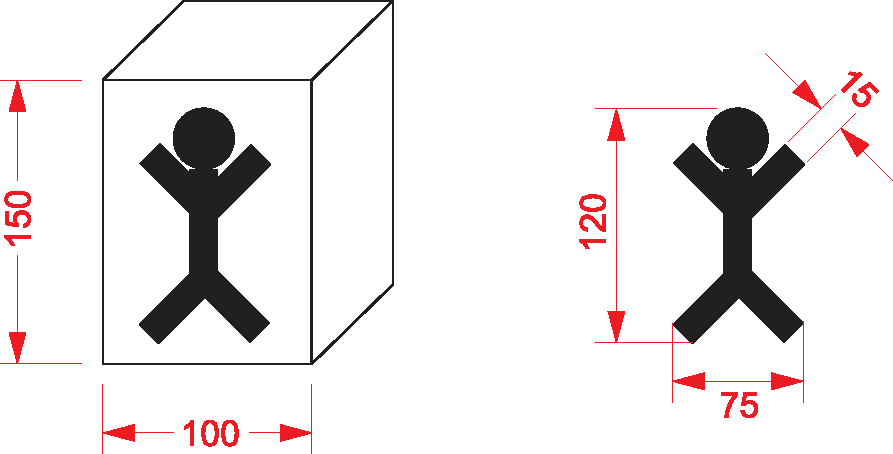
\includegraphics[]{graphics/Abb_21_pedestrians.pdf}
\end{center}
\end{figure}

\section{Example Circuit}
\label{fig_example_circuit}
\vspace*{2cm}
\begin{figure}[H]
\begin{center}
	\centering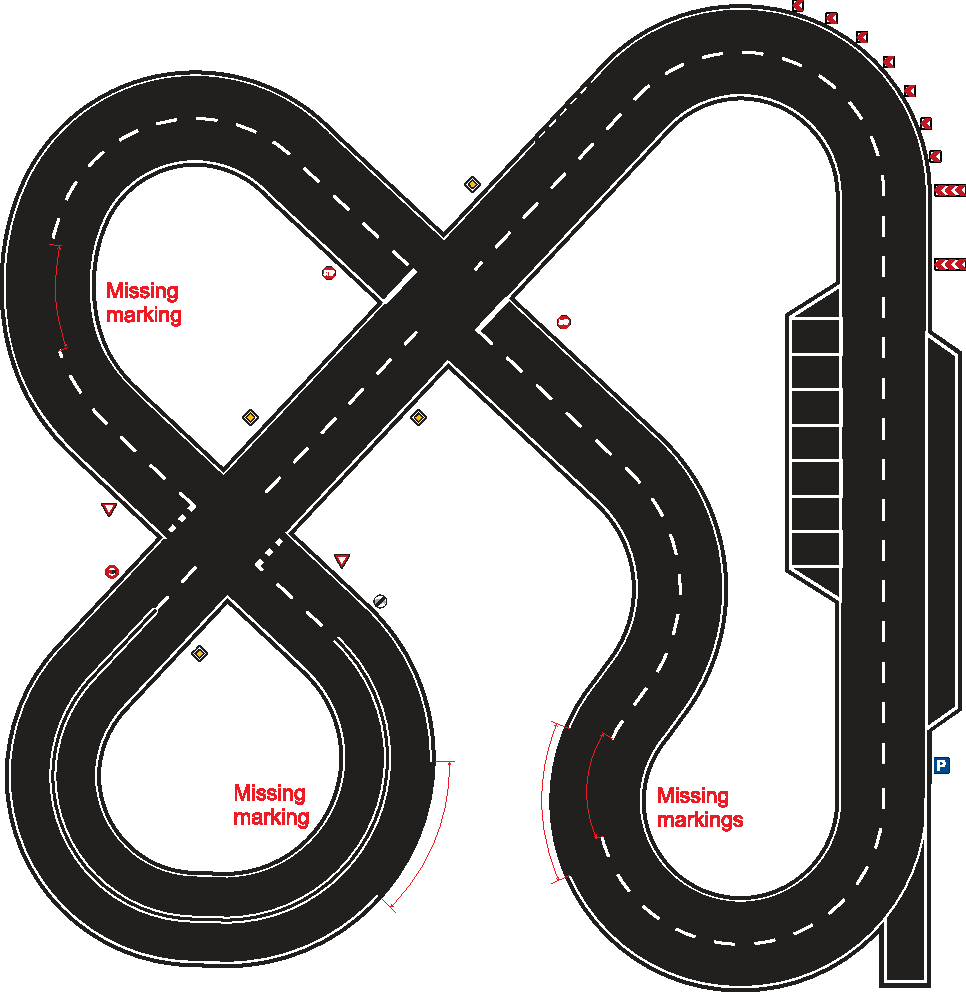
\includegraphics[width=\textwidth]{graphics/Abb_22_example_circuit.pdf}
\end{center}
\end{figure}

\section{Markings of the Start Box Gate}
\label{fig_start_box_markings}
\begin{figure}[H]
\begin{center}
	\centering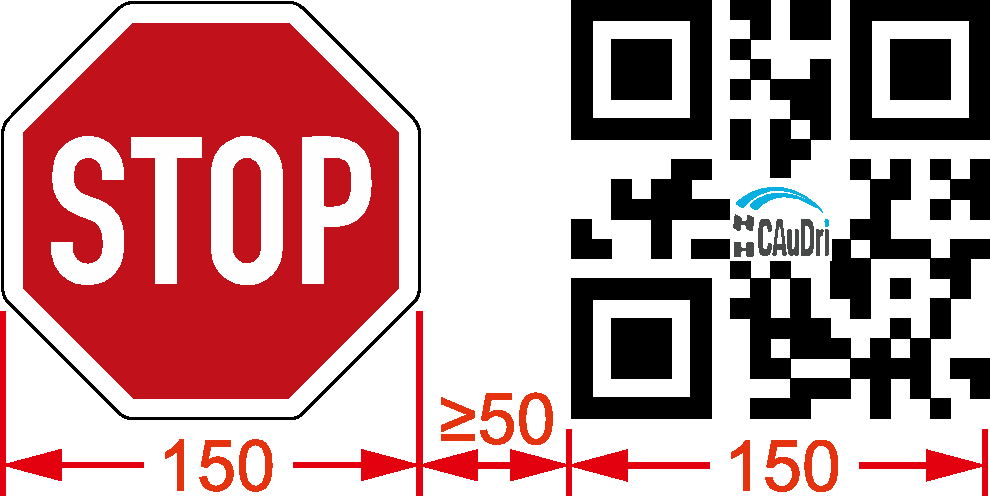
\includegraphics[width=\textwidth]{graphics/Abb_23_start_box_markings.pdf}
\end{center}
\end{figure}




\end{document}